\section{System architecture}
\label{sec:sys_arch}

The developed 3D/4D GIS system has a two-tier {\em client-server} architecture (Figure \ref{fig:sys_arch_2tier}). The {\em server} contains the master copy of the data and a PostgreSQL database called \textit{viaappiadb}. The {\em clients} download or request the data required for visualization and run the 3D/4D viewer locally or via a Web application which connects to the remote database when required.
 
A diagram of the data preparation framework which is executed in the server is shown in Figure \ref{fig:sys_arch_data_framework}. The acquired data for the road itself (background) are usually point clouds, while for the monuments (sites) the data are of more modalities- point clouds, meshes, pictures. Depending on the prefered application on the client side, Windows desktop or Web-based, the raw data are handled in one of the two ways. 

In the former case the raw data is converted to the binary format of the OpenSceneGraph (\url{http://www.openscenegraph.org}). In the latter case, the point clouds are converted using the POTREE (\url{potree.org}) WebGL point cloud converter. The \textit{viaappiadb} database is filled with meta-data information of the location of the raw data and the converted data. The archaeological information with attribute data for the several sites is provided in a Microsoft Access file. It needs to be converted to the PostgreSQL format before being imported into the main database. The footprints (and the alritute range??) are provided in a PostgreSQL dump file and are imported into the \textit{viaappiadb} database as well. On Figures \ref{fig:sys_arch_data_framework} and \ref{fig:sys_arch_2tier} the solid arrows indicate data flow, while the dashed arrows indicate metadata flow.

\begin{figure}[!ht]
 \centering
 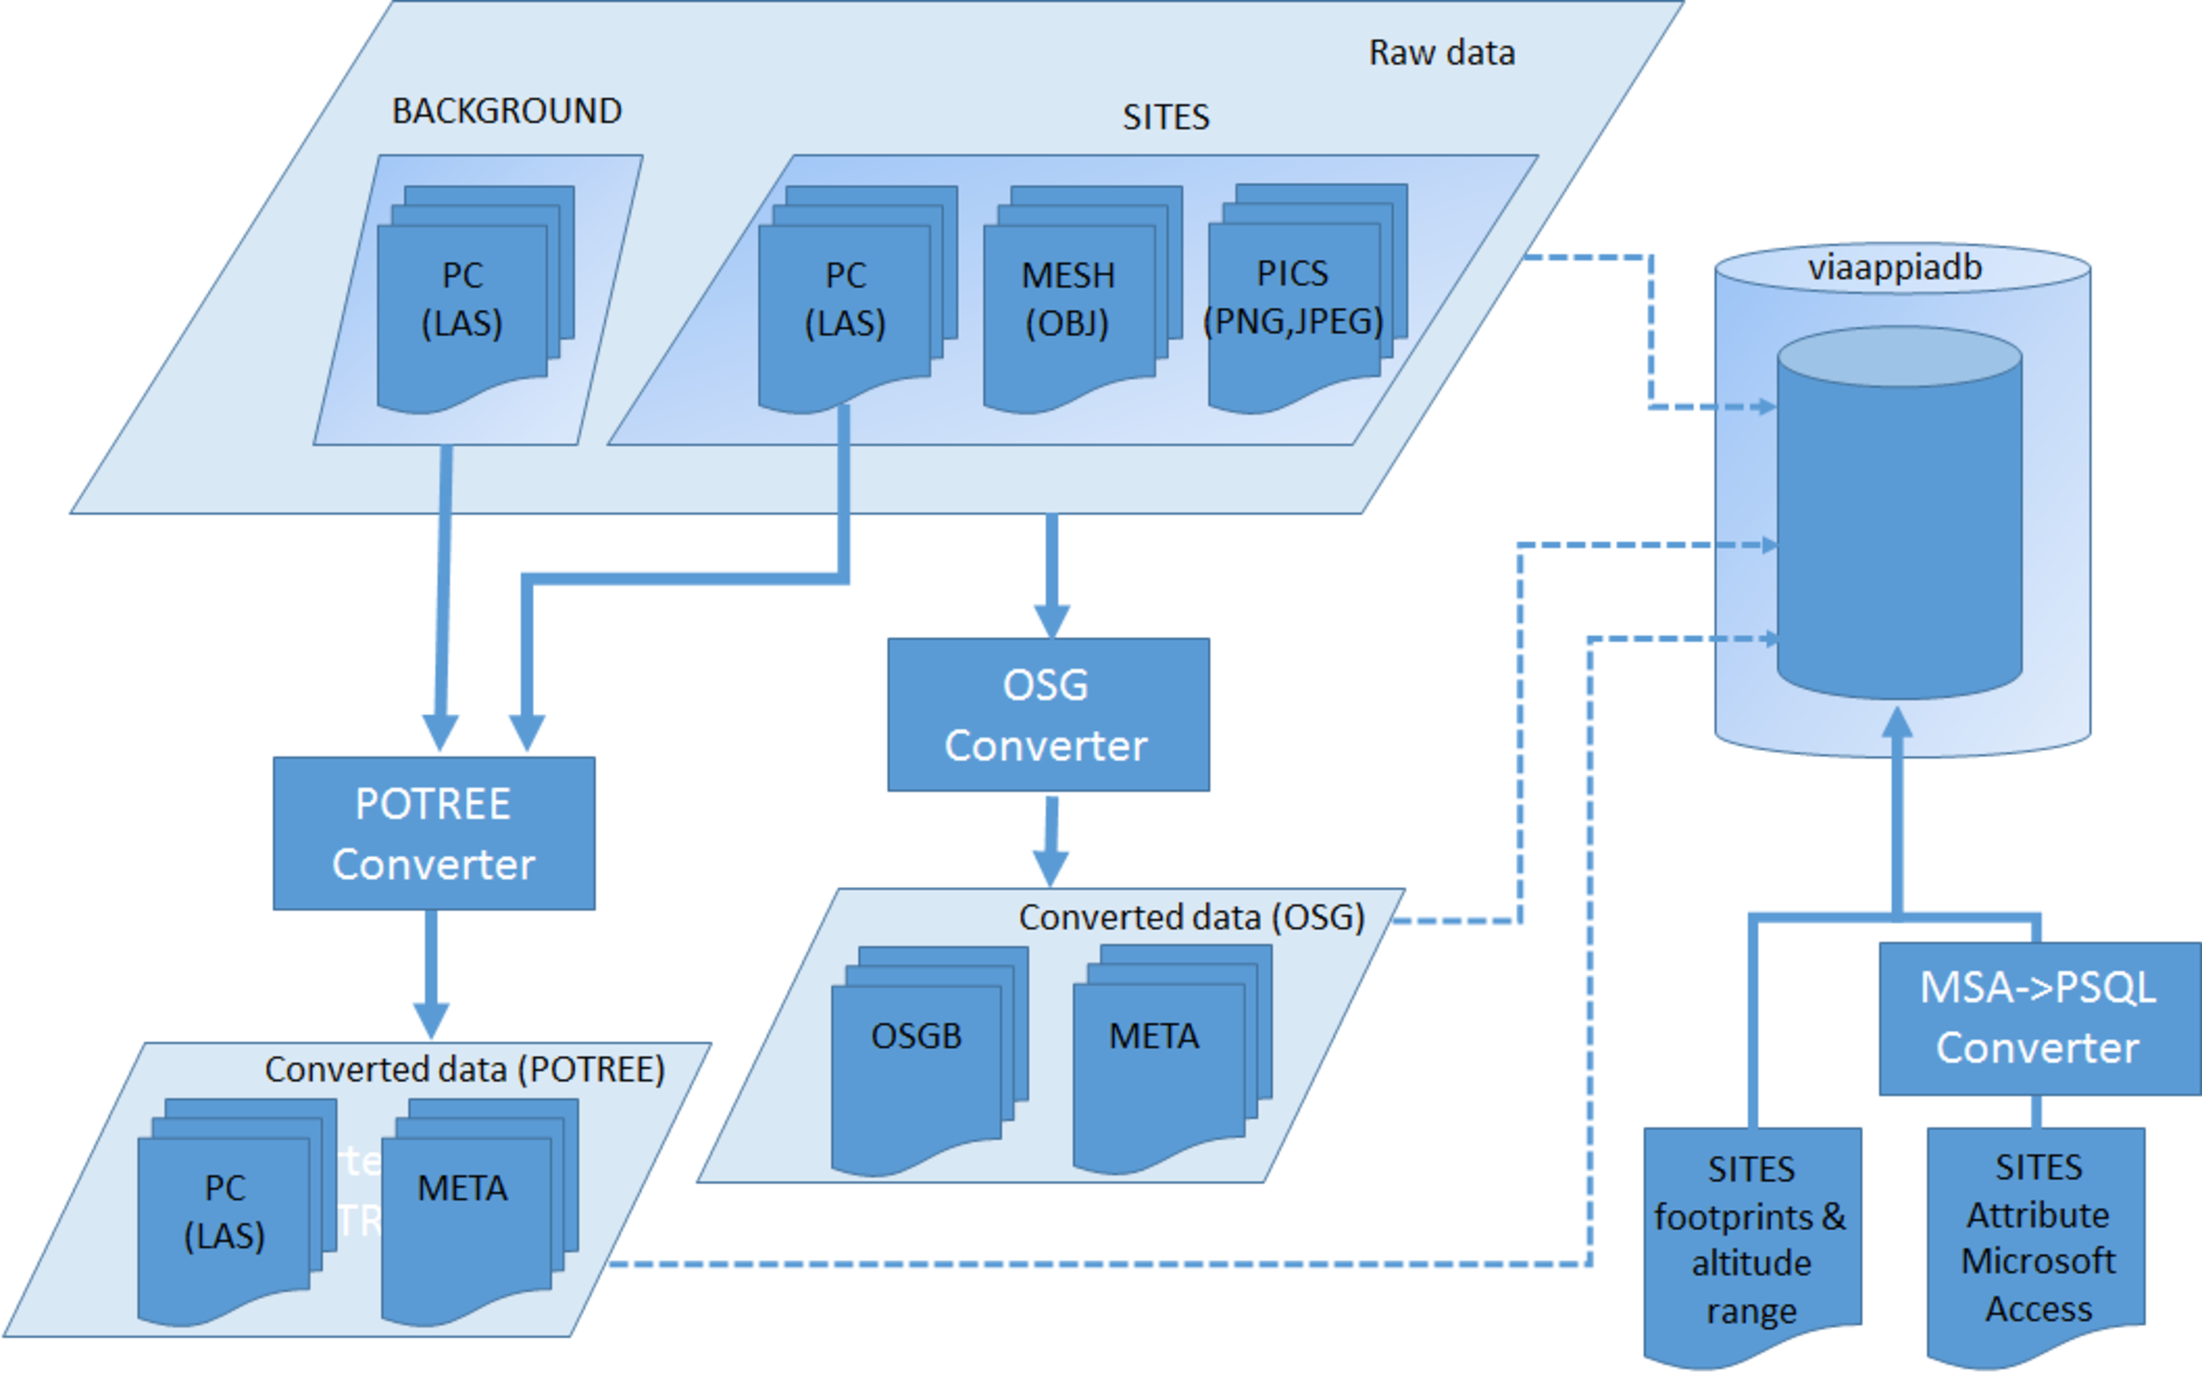
\includegraphics[width=0.75\textwidth]{fig/system_architecture/DataFramework.pdf}
 \caption{}
 \label{fig:sys_arch_data_framework}
\end{figure}

\begin{figure}[!ht]
 \centering
 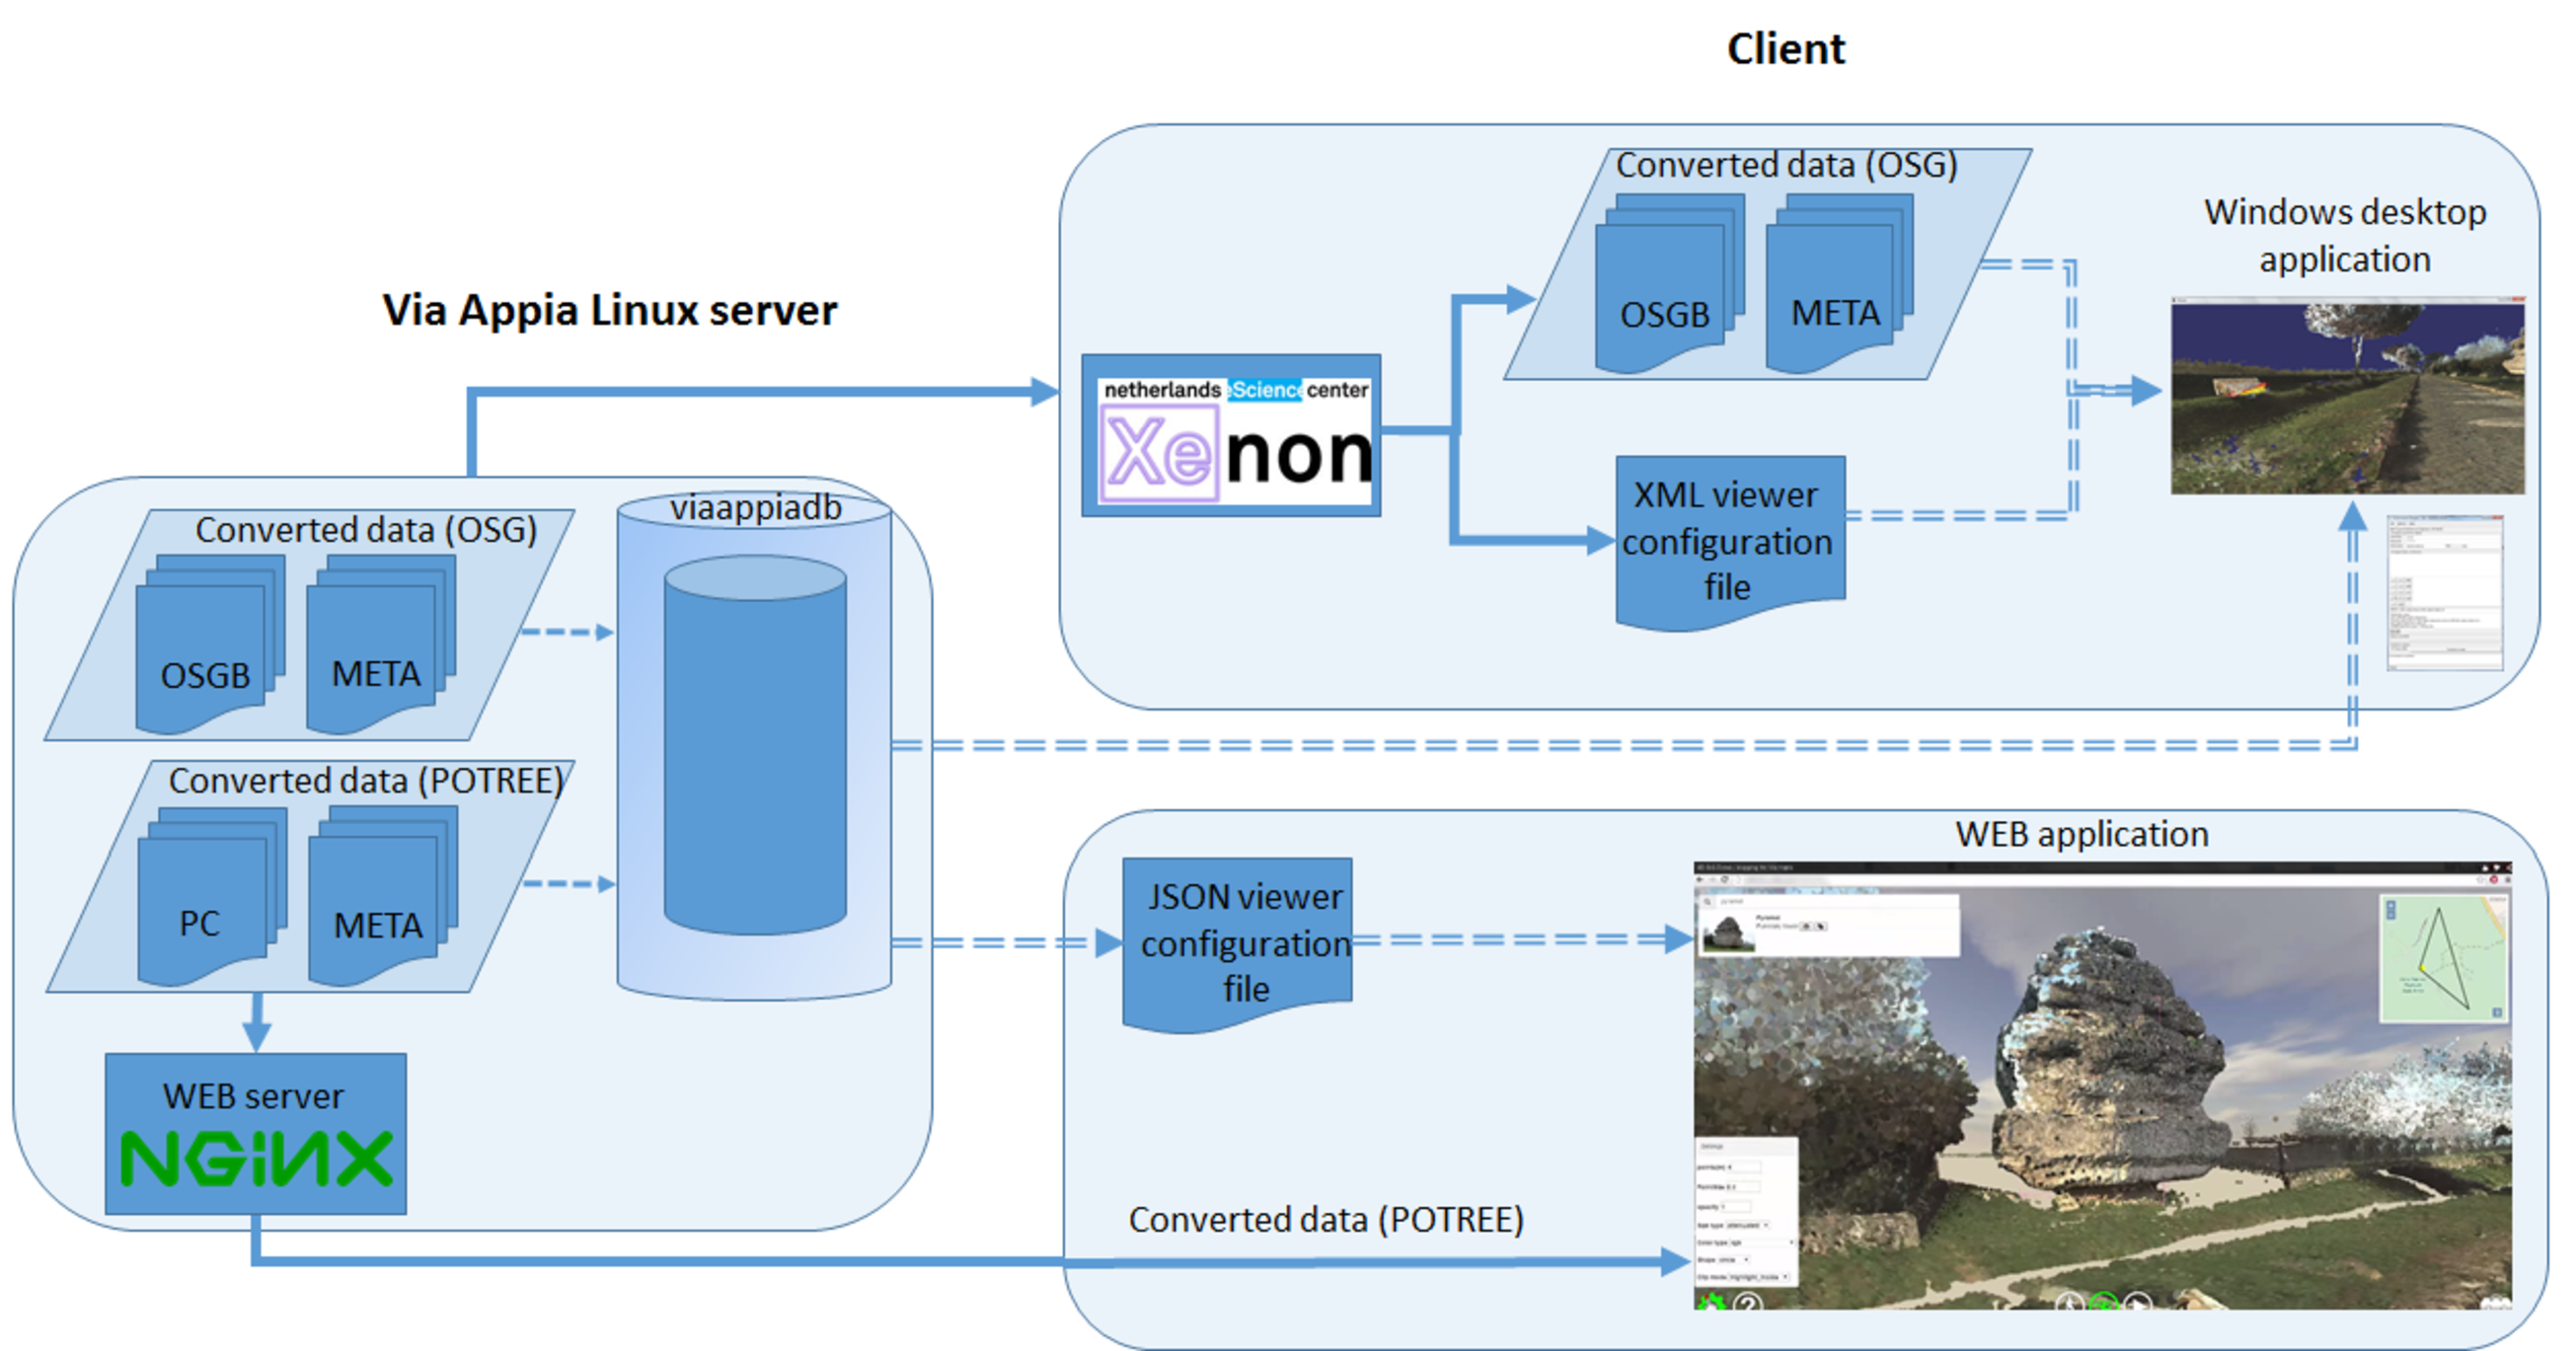
\includegraphics[width=0.95\textwidth]{fig/system_architecture/TwoTierArchitecture.pdf}
 \caption{}
 \label{fig:sys_arch_2tier}
\end{figure}